\chapter{Theoretical Background}

\section{The model}

\subsection{L\'evy walks}

The original motivation for the creation of the L\'evy walk model goes back to the work of Richardson in 1926 \cite{richardson}, who studied the motion of particles in the turbulent flow of the atmosphere. Such a system contains jets and eddies that affect the behavior of the particle and lead to anomalous diffusion. In particular Richardson found that the \gls{msd} of the particle scales with the third power of the time, i.e.

\begin{align}
\gls{x2}(t) \propto t^3 ,
\end{align}
%
which is known as the Richardson regime.\\

There were several attempts to find a random walk model that replicates this behavior. These attempts found that power-law models were particularly suitable for describing superdiffusion \footnote{meaning diffusion where $\gls{x2}(t) \propto t^{1+\alpha}$, $\alpha>0$} which lead to the creation of the L\'evy flight model: In this model the walker jumps instantaneously in a random direction with a jump length drawn from a distribution $g(\abs{\ve{x}})$. He now waits at the turning point for the duration of the waiting time, which is drawn from the distribution $\gls{psi}(t)$ and then performs a new jump in another direction, as can be seen in figure (\ref{fig:levyFlight}). Both the waiting time and the jump length distributions are power-laws, meaning for large arguments they take the form 

\begin{align}
\gls{psi}(t) \propto t^{-1-\gamma}, \qquad g(\abs{\ve{x}}) \propto \abs{\ve{x}}^{-1-\beta}, \qquad \gamma, \beta > 0.
\end{align} 
%
\begin{figure}
\begin{center}
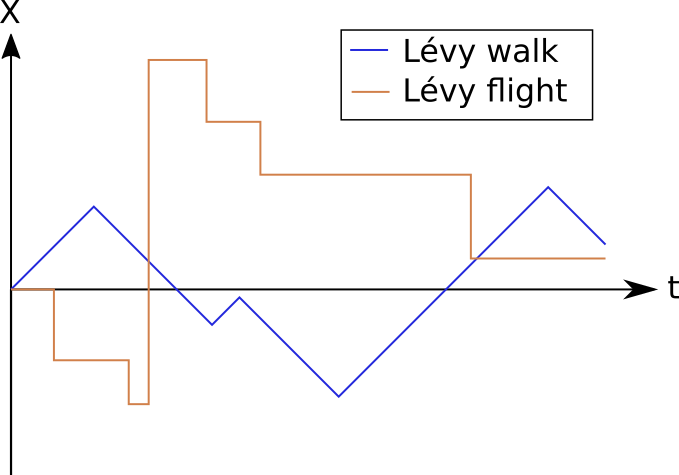
\includegraphics[width=90mm]{pics/levyFlight.png}
\caption{Comparison between the trajectories of the one dimensional L\'evy flight and L\'evy walk (for $\nu=1$). Note that the jump length of the L\'evy flight is independent of the waiting time. 
\label{fig:levyFlight}}
\end{center}
\end{figure}
%
However the L\'evy flight model has a major drawback: Since the jumps happen instantaneously it has an infinite propagation speed, which causes its \gls{msd} and all higher moments to diverge \cite{lwreview}. \\


Therefore the L\'evy walk model was developed by Shlesinger, Klafter and West \cite{shlesinger1987}. Here the walker no longer waits at the turning points, but his jumps now have a finite duration, turning them into steps. The step duration is coupled to the length of the step and prevents the infinite propagation speed that caused problems with the L\'evy flights, which is illustrated in figure \ref{fig:levyFlight}. \\

The path of a walker in the new model is now described by a series of step durations $\gls{dur}_1, \gls{dur}_2, ...$ which are drawn from the power-law distribution 

\begin{align}
\gls{psi}(\gls{dur}_i) = \frac{\gamma}{t_0} \frac{1}{(1+\gls{dur}_i/t_0)^{\gamma+1}} .
\end{align}
%
Here the parameter $\gamma>0$ governs the width of the distribution and { \color{red}$t_0$ is the timescale of a step }. These step durations are associated with their respective steps vectors $\ve{x}_1, \ve{x}_2, ...$, whose direction is chosen randomly. By partially summing up the step durations and the step lengths one obtains the turning times $\gls{ttime}_n$ and the turning points $\gls{tpoint}_n$ respectively:

\begin{align}
\gls{ttime}_n = \sum_{j=1}^n \gls{dur}_j , \qquad \gls{tpoint} = \sum_{j=1}^n \ve{x}_j
\end{align}
%
The walker is now being observed at the observation time $t$: Let the last turning time before $t$ be $\gls{ttime}_n = \text{ max} \{\gls{ttime}_i | \gls{ttime}_i \leq t \}$, then the distance covered from the last turning point is given by

\begin{align}
\abs{\ve{x}_{n+1}} = c (\gls{dur}_{n+1})^{\nu-1} (t-\gls{ttime}_n) ,
\end{align}
%
where c is a constant with dimension $ [ s t^{-\nu} ] $ . The speed 

\begin{align}
\gls{speed} = \pder{}{t} \abs{\ve{x}_{n+1}} = c (\gls{dur}_{n+1})^{\nu-1}
\end{align}
%
is therefore constant during the entire step but depends on the step duration $\gls{dur}_{n+1}$, where the parameter $\nu>0$ governs this dependence. \\
For any completed step we can now write down the joint probability to make a step of length $\abs{\ve{x}}$ and duration $\gls{dur}$:

\begin{align}
\gls{psi}(\ve{x}, \gls{dur} ) = \frac{\gamma}{t_0} \frac{1}{(1+\gls{dur}/t_0)^{\gamma+1}}  \frac{\delta(\abs{\ve{x}} - c \gls{dur}^{\nu}) }{\abs{\gls{step}}^{d-1} \abs{S^{d-1}}}  .
\end{align}
%
Here $d$ is the spatial dimension of the process and $\abs{S^{d-1}}$ is the surface area of a d-dimensional unit ball. Note that both the step duration distribution and the joint distribution are denoted by $\gls{psi}$, but their arguments are different. In conclusion we have a model that is governed by two parameters, $\nu$ and $\gamma$ and can produce different kinds of anomalous diffusion.\\

Because of this versatility the L\'evy walk model is used to describe a variety of systems: Besides the application in turbulent systems for which the model was originally invented it finds application in field like biology, where  the special case of fixed velocities ($\nu=1$) is used to approximate the motion of E. coli bacteria, who move with the help of microscopic flagella. These flagella either rotate in a synchronized manner, which leads to long stretches of relatively fast movement, or unsynchronized, which leads to a tumbling motion in which the bacterium changes its direction. The resulting motion was found to follow a power-law distribution with parameter $\gamma = 1.2$ \cite{korobkova2004}

\todo{more examples: light scattering, chaotic Hamiltonian systems}



However it was found recently in \cite{radons2018} that the \gls{msd} of the model is actually divergent for certain values of its parameters, a fact that had previously gone unnoticed for the three decades of the models existence. 
The divergence can be seen directly when one writes down the contribution to the second moment of the distribution from the trajectories, that consist only of a single step longer than the observation, i.e. where the particle never stops:

\begin{align}
\gls{x2}(t) \geq& \int_{\mathbb{R}^d} \int_{t}^{\infty} \abs{\gls{step}}^{2}(t') \gls{psi}(\gls{step},t') dt' d^{d}x \\
=& \frac{\gamma}{t_0} \int_{0}^{\infty} \int_{t}^{\infty} \abs{\gls{step}}^{2}(t')  \frac{1}{(1+t'/t_0)^{\gamma+1}}  \delta(\abs{\gls{step}} - c (t')^{\nu-1}t)  dt' d\abs{\gls{step}} \\
=& \frac{\gamma t^2}{t_0}  \int_{t}^{\infty}   \frac{c^2 (t')^{2\nu-2}}{(1+t'/t_0)^{\gamma+1}}    dt'  .
\end{align}
%
The integrand is proportional to $(t')^{2\nu-\gamma-3}$, therefore the integral will diverge at infinity whenever $2 \nu \geq \gamma +2$ holds. This includes the parameter region where the Richardson regime was expected, so the model that was essentially invented to cure the divergence in the description of the Richardson regime turns out to be divergent itself. In order to remedy this, a more general model model is necessary, whose investigation will be the focus of this thesis.
% problem: divergence from radons

\subsection{Generalized L\'evy walks}

%mention drude model of Sokolov
% interpolation via eta
% formulate model 
% picture
% general properties

% Further generalizations of the model

\section{Theory of random walks}

\subsection{Continuous time random walks}

%zoom in from RW -> CTRW -> space-time coupled CTRWs

% introduce laplace tf

% introduce: survival probability, forward waiting time, step rate, mean number of steps 

% derive formula for number of steps 

% derive formula for total pdf

\subsection{Space-time coupled continuous time random walks}

